\documentclass[25pt, a1paper, landscape, innermargin=-3in]{tikzposter}

% required packages
\usepackage{amsmath}
\usepackage{amsfonts}
\usepackage{amsthm}
\usepackage{graphicx}
\usepackage[square,numbers]{natbib}
\usepackage{url}
\usepackage{booktabs}
\usepackage{geometry}

% set the appropriate paper size
\geometry{papersize={40in,42in}}

% compact bibliography
\renewcommand{\bibsection}{}
\setlength{\bibsep}{0pt plus 0.3ex}

%% Available themes: see also
%% https://bitbucket.org/surmann/tikzposter/downloads/themes.pdf

\definecolorpalette{sampleColorPalette} {
  \definecolor{colorOne}{named}{green}
  \definecolor{colorTwo}{named}{black}
  \definecolor{colorThree}{named}{cyan}
}
\usetheme{Default}
%% \usecolorstyle{Denmark}
\colorlet{backgroundcolor}{white}
\colorlet{framecolor}{gray}
\colorlet{blocktitlebgcolor}{gray}

% title information
\title{Guidance on Individualized Treatment Rule Estimation in High Dimensions}
\author{Philippe Boileau$^1$, Ning Leng$^2$, Sandrine Dudoit$^3$}
\institute{$^1$McGill University; $^2$Genentech Inc; $^3$University of California, Berkeley}

% dictate default block options
\newcommand{\myblock}[2]{\block[titleinnersep=2mm, linewidth=0.5mm]{#1}{#2}}
\newcommand{\mysmallblock}[2]{\block[titleinnersep=1mm, linewidth=1mm, bodyinnersep=5mm, roundedcorners=12, ]{{\small #1}}{{\scriptsize#2\par}}}

% turn off
\tikzposterlatexaffectionproofoff
\begin{document}
\maketitle[width=34in]


\begin{columns}

  \column{0.333}

  \myblock{Motivation}{

    Precision medicine promises to tailor patients' treatments to optimize their
    outcomes. Patients' pre-treatment covariates, like age, sex-at-birth, and
    genetic profiles, influence therapies' efficacy, safety, and tolerability
    outcomes. These patient characteristics, known as \textbf{treatment effect
      modifiers, are used to derive individualized treatment rules (ITRs) that
      guide personalized treatment decisions}.

    \vspace{0.1in}

    While numerous methods can successfully estimate ITRs in traditional
    asymptotic settings, \textbf{learning ITRs from high-dimensional data with
      more pre-treatment covariates than patients --- a common occurrence in
      modern clinical data --- is challenging}. ITR estimators developed for
    such data rely on simplifying assumptions. Recent advances in
      treatment effect modifier detection may help.

    \vspace{0.1in}

    A comparison of available methods has not been performed. Nor has an
    evaluation of these methods' sensitivity to assumption violations. As such,
    \textbf{selecting an appropriate ITR estimation strategy for
      high-dimensional settings is challenging for applied biomedical
      researchers}. Capacity for precision medicine is diminished as a result.

  }

  \myblock{Primary Objectives}{
    \begin{itemize}
        \item \textbf{Provide guidance based on practical operating
          characteristics to applied scientists for ITR estimation in high
          dimensions.}
        \item \textbf{Determine whether treatment effect modifier detection
          procedures improve ITR estimation in high-dimensions.}
    \end{itemize}
  }

  \myblock{Operating Characteristics}{
    \begin{itemize}
        \item \textbf{Rule Quality:} An ITR is ``high-quality'' when its
          expected outcome approaches that of the optimal rule. That is, the
          rule approximately optimizes mean outcome in the population.

        \item \textbf{Accurate Interpretability:} An ITR is accurately
          interpretable when it recovers treatment effect modifiers reliably in
          terms of the false discovery, true positive, and true negative rates.

        \item \textbf{Computational Efficiency:} An ITR is computationally
          efficient when it can be estimated quickly in serial with few
          computational resources.

    \end{itemize}
  }

  \myblock{Problem Formulation}{

    Consider $n$ i.i.d.~observations $O = (W, A, Y)$ where $W$ is a $p$-length
    random vector of pre-treatment covariates (and possible confounders) where
    $p \approx n$ or $p > n$, $A$ is a binary treatment indicator, and $Y$ is
    the continuous outcome.

    \vspace{0.1in}

    We aim to estimate the ITR, defined as
    \begin{equation*}
      I(\mathbb{E}[Y|W, 1] - \mathbb{E}[Y|W, 0] > 0) \;,
    \end{equation*}
    where $\mathbb{E}[Y|W, 1] - \mathbb{E}[Y|W, 0]$ is the conditional average
    treatment effect (CATE) under standard identifiability
    conditions.

  }

  \mysmallblock{References}{
    \bibliographystyle{unsrtnat}
    \bibliography{refs}
  }

  \column{0.334}

  \myblock{Estimators}{

    The CATE estimators in the table below were used to construct ITR
    estimators. Filtered versions of these CATE estimators relying on the
    treatment effect modifier variable importance parameter methodology of
    \citet{boileauNonparametricFrameworkTreatment2025} were used to construct
    ITR estimators as well.

    \begin{tikzfigure}
      \centering
        \begin{tabular}{
            |p{3in} || p{8.5in}|
          }
          \hline
          CATE Estimator
          & Details \\
          \hline\hline
          Plug-In LASSO
          & A plug-in estimator using the LASSO \citep{tibshiraniRegressionShrinkageSelection1996}. \\
          \hline
          Plug-In XGBoost
          & A plug-in estimator using XGBoost \citep{chenXGBoostScalableTree2016}. \\
          \hline
          Modified Covariates LASSO
          & A modified covariates estimator \citep{tianSimpleMethodEstimating2014} using the LASSO. The propensity
          score is estimated using the logistic LASSO. \\
          \hline
          Modified Covariates XGBoost
          & A modified covariates estimator
          \citep{tianSimpleMethodEstimating2014} using XGBoost. The propensity
          score is estimated using the logistic LASSO. \\
          \hline
          Augmented Modified Covariates LASSO
          & An augmented modified covariates estimator
          \citep{tianSimpleMethodEstimating2014} using the LASSO. The propensity
          score is estimated using the logistic LASSO. \\
          \hline
          Augmented Modified Covariates XGBoost
          & An augmented modified covariates estimator
          \citep{tianSimpleMethodEstimating2014} using XGBoost. The propensity
          score is estimated using the logistic LASSO. \\
          \hline
          AIPW-based LASSO
          & An AIPW-based estimator
          \citep{luedtkeSuperLearningOptimalDynamic2016} using Super Learners
          \citep{laanSuperLearner2007} to estimate the
          expected conditional outcome and the propensity score. Differences
          in predicted pseudo-outcomes are modelled using the LASSO. \\
          \hline
          AIPW-based Super Learner
          & An AIPW-based estimator
          \citep{luedtkeSuperLearningOptimalDynamic2016} using Super Learners to estimate the
          expected conditional outcome and the propensity score. Differences
          in predicted pseudo-outcomes are modelled using a Super Learner. \\
          \hline
          Causal Random Forests
          & A causal random forest estimator
          \citep{wagerEstimationInferenceHeterogeneous2018} using
          cross-validation for hyperparameter selection. \\
          \hline
      \end{tabular}
    \end{tikzfigure}

  }

  \myblock{Simulated Data-Generating Processes}{

    ITR estimators were benchmarked on 16 data-generating processes with
    continuous outcomes and binary treatment assignments reflecting a diversity
    of randomized and observational studies. Realizations of random vector $O$
    with $p=500$ were generated according to the data-generating process
    template:
    \begin{align*}
      W & \sim N(0, \Sigma) \\
      A|W & \sim \text{Bernoulli}(\pi(W)) \\
      Y|W, A & \sim N(\mu(W, A), 1) \;.
    \end{align*}
    Here, $\Sigma$ is some $500 \times 500$ covariance matrix,
    $\pi(W)=\mathbb{P}[A=1|W]$, and $\mu(W,A) = \mathbb{E}[Y|W, A]$. Sixteen
    data-generating processes are defined using combinations of the following
    factors:
    \begin{equation*}
      \begin{split}
        \Sigma_{1} & = I_{500 \times 500} \\
        \Sigma_{2} & = \text{Block diagonal} \\
      \end{split}
    \end{equation*}
    \begin{equation*}
      \times
    \end{equation*}
    \begin{equation*}
      \begin{split}
        \pi_{1}(W) & = \frac{1}{2} \\
        \pi_{2}(W) & = \text{logit}^{-1}\left(\frac{W_{1} + W_{2} + W_{3} + W_{4}}{5}\right) \\
      \end{split}
    \end{equation*}
    \begin{equation*}
      \times
    \end{equation*}
    \begin{equation*}
      \begin{split}
        \mu_{1}(A, W) & = A + \gamma^{\top}W + (\delta^{(10)})^{\top}WA \\
        \mu_{2}(A, W) & = A + \gamma^{\top}W + (\delta^{(50)})^{\top}WA \\
        \mu_{3}(A, W) & = \gamma^{\top}W + 2\;\text{arctan}\left\{(\delta^{(10)})^{\top}WA\right\} \\
        \mu_{4}(A, W) & = \gamma^{\top}W + 2\;\text{arctan}\left\{(\delta^{(50)})^{\top}WA\right\} \\
      \end{split}
    \end{equation*}

  }

  \column{0.333}

  \myblock{Results Snapshot}{
    \vspace{-0.5in}

    \begin{tikzfigure}
      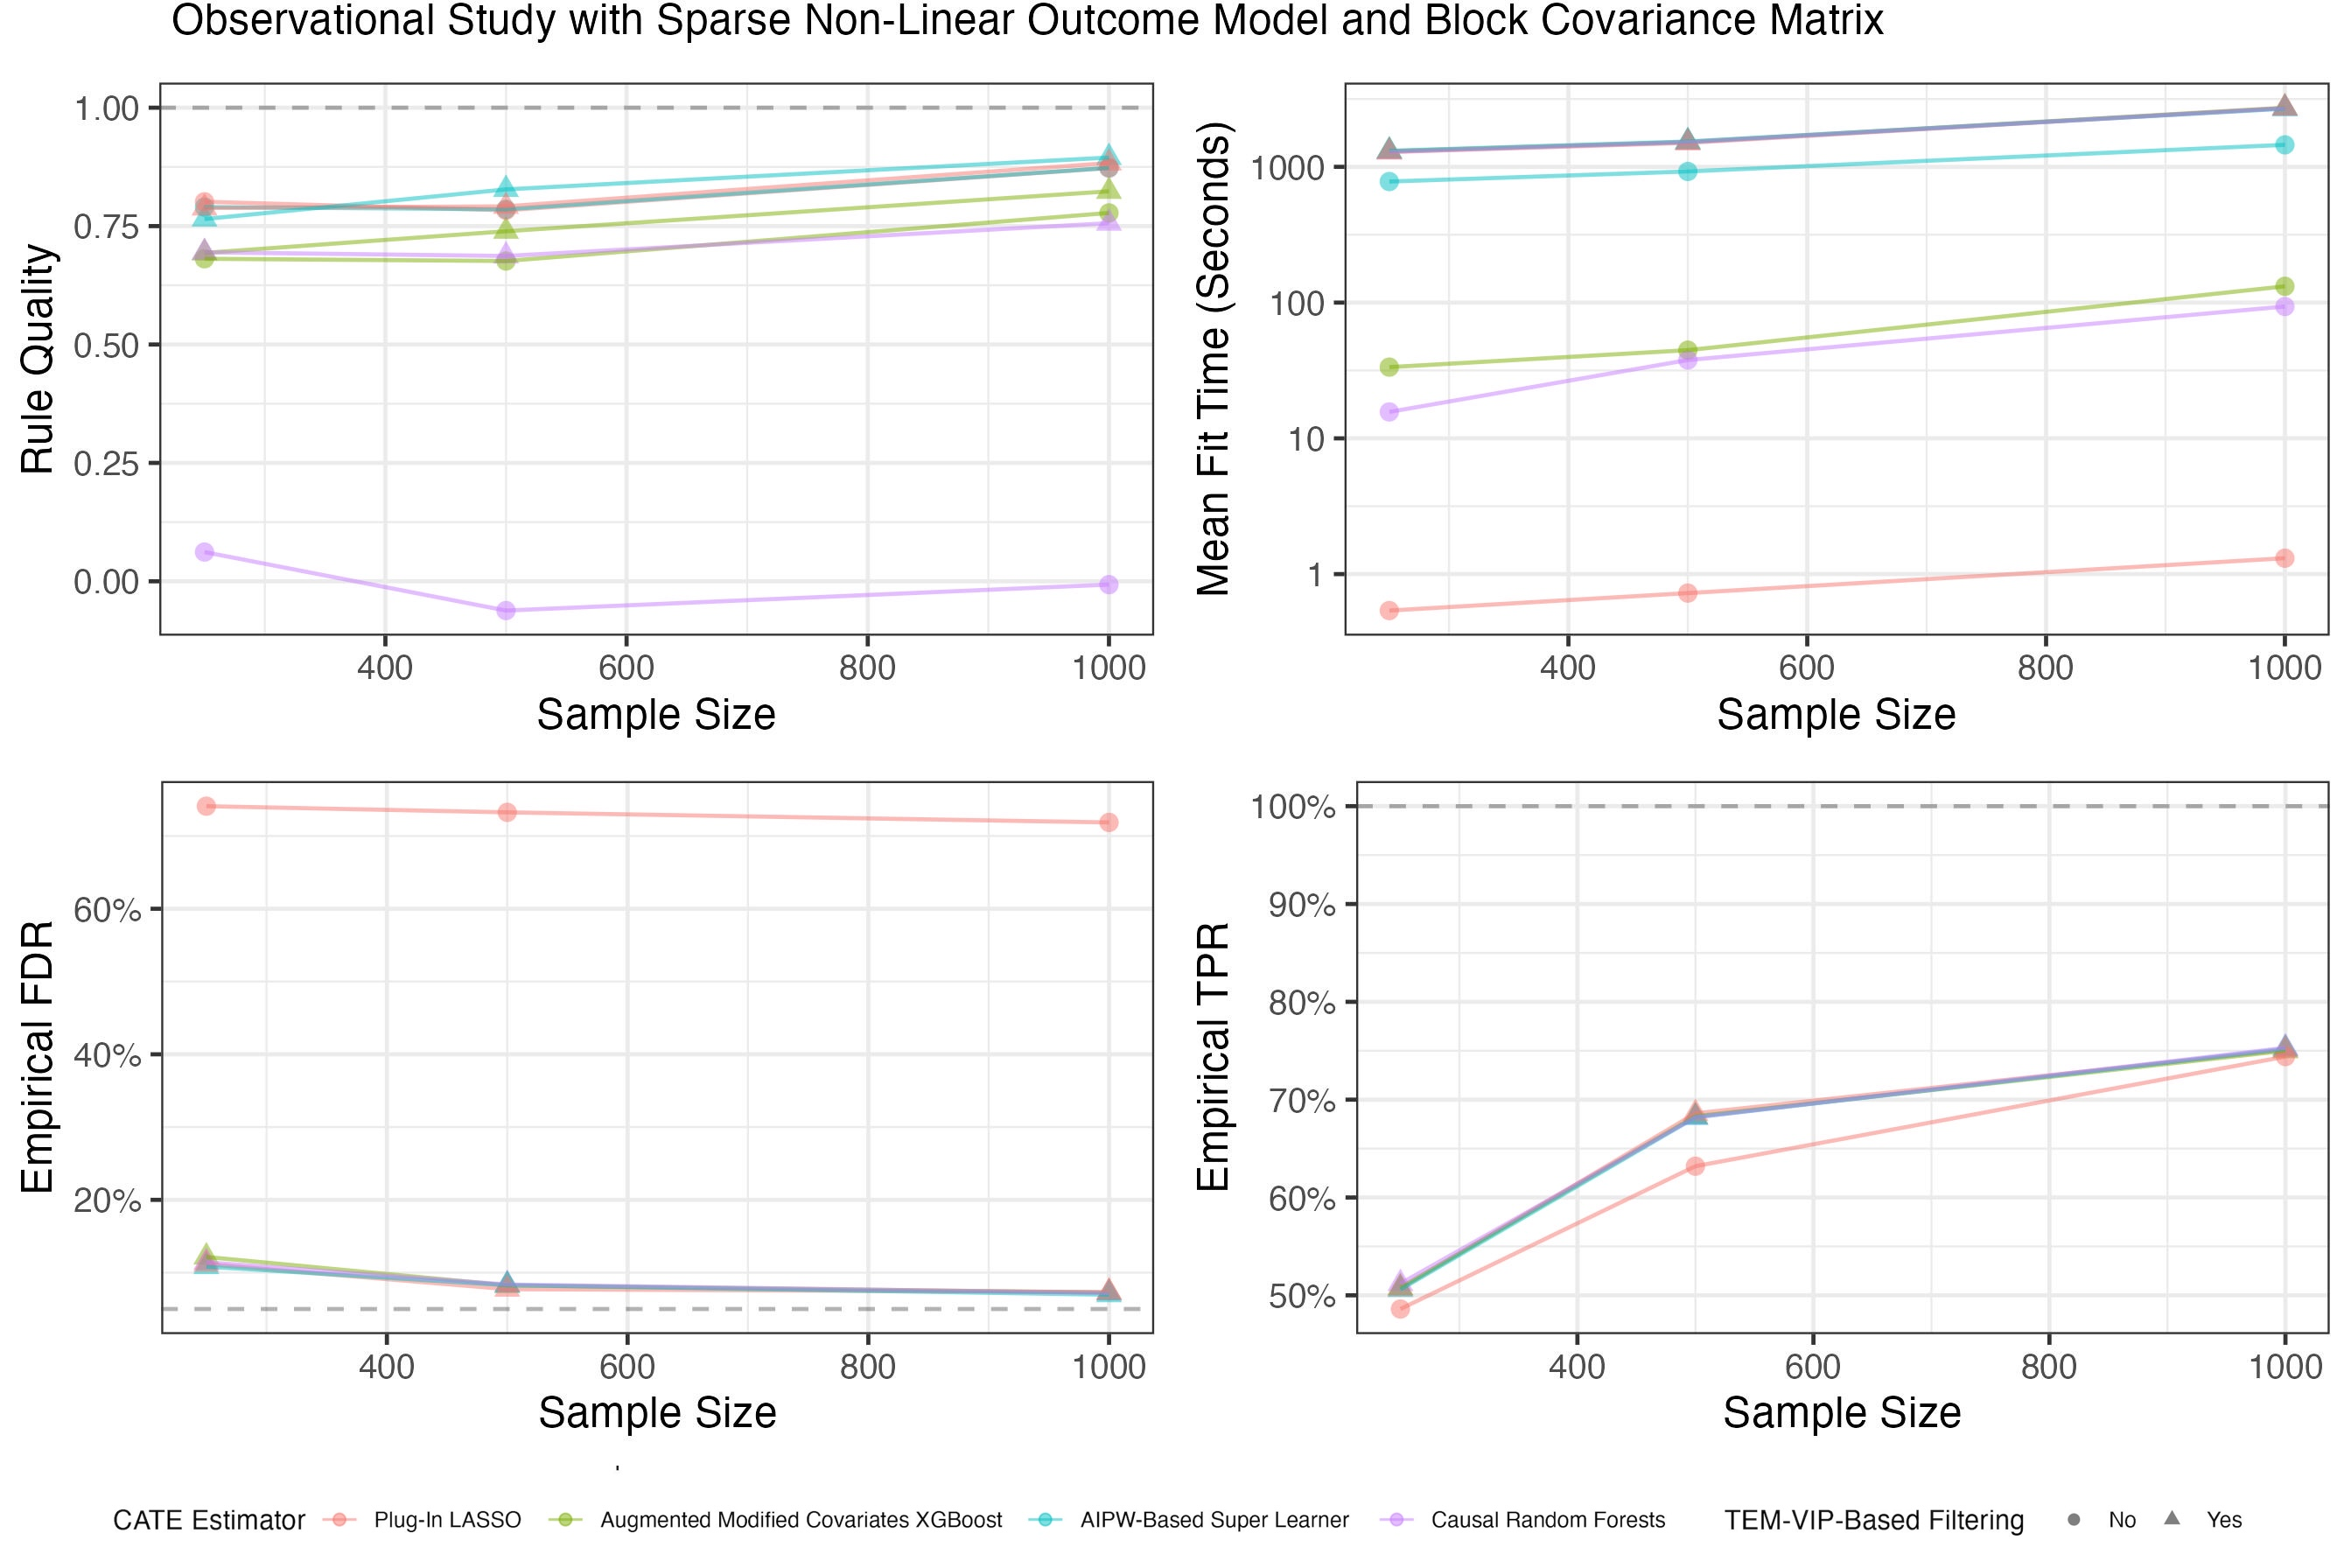
\includegraphics[width=0.28\textwidth]{figs/summary-plot.jpeg}
    \end{tikzfigure}

    \vspace{-0.2in}

  }

  \myblock{Practical Guidance}{

    \textbf{No estimator uniformly dominates others across all operating
      characteristics; tradeoffs must be made.} Since rule quality is generally
    of primary concern, practitioners must choose between accurate
    interpretability and computationally efficiency. We provide the following
    guidance on this tradeoff when selecting an ITR estimator for
    high-dimensional data:

    \begin{itemize}

    \item \textbf{High-quality ITRs that are accurately interpretable:} The
      filtered LASSO-based plug-in and AIPW-based estimators generally produce
      high-quality ITR estimates while accurately recovering TEMs. These
      estimators are computationally intensive, however. The computational
      burden might be lestned by parallelizing the estimation procedure.

    \item \textbf{High-quality ITRs that require few computational resources:}
      The LASSO-based plug-in estimator produces among the most high-quality
      rules in our simulation studies, providing empirical evidence that it is
      robust to model misspecification while being exceptionally computationally
      efficient. This estimator's built-in feature selection capabilities should
      not be used for TEM discovery, however.

    \end{itemize}
  }

  \begin{subcolumns}
    \subcolumn{0.8}

    \mysmallblock{Funding}{

      P.B. gratefully acknowledges the support of the Fonds de recherche du
      Québec - Nature et technologies and the Natural Sciences and Engineering
      Research Council of Canada.

    }
  \end{subcolumns}


\end{columns}

\node [above left, outer sep=2cm] at (bottomleft -| topright) {
\includegraphics[width=6cm]{logos/qr-code}};

\end{document}
